% !TeX root = ../main.tex
\section{Garbage collection}

Every heap-allocated value we've discussed in this block, boxed integers, closure
records, activation records that escape their frame, has to be reclaimed \emph{sometime},
or the program's memory usage grows without bound. This section is about who's
responsible for that reclamation, and what happens when you get it wrong.

\subsection{manual memory management's failure modes}

The straightforward answer is: the programmer decides when a value is done being used,
and frees it explicitly. This is simple to explain and genuinely fast when done right,
but it has three classic ways to go wrong.

\begin{lstlisting}[language=C]
int *p = malloc(sizeof(int));
*p = 42;
/* ... p is never freed ...  */             /* memory leak */

int *q = malloc(sizeof(int));
free(q);
printf("%d\n", *q);                          /* use-after-free: q is dangling */

int *r = malloc(sizeof(int));
free(r);
free(r);                                     /* double free */
\end{lstlisting}
A \textbf{memory leak} is memory that's no longer reachable by the program but was
never freed, it just sits there, unusable and unreclaimed, for the rest of the
program's run. A \textbf{dangling pointer} / \textbf{use-after-free} is the opposite
mistake, freeing memory too early and then reading (or writing) through a pointer that
still refers to it, memory that may since have been reused for something else entirely.
A \textbf{double free} corrupts the allocator's own internal bookkeeping by freeing the
same block twice. All three are notoriously hard to catch by inspection, and all three
are exactly what \textbf{garbage collection} (GC) exists to make structurally
impossible: instead of trusting the programmer to track ownership by hand, the runtime
figures out automatically when a value can no longer be used, and only then reclaims
it.

\subsection{reference counting}

The simplest automatic scheme: every heap object carries a count of how many references
point to it. Creating a new reference increments the count; a reference going out of
scope or being overwritten decrements it; when the count hits zero, nothing can reach
the object anymore, so it's freed immediately.

\begin{remark}
Reference counting's big appeal is that reclamation is \emph{incremental} and
\emph{immediate}, memory is freed the instant it becomes unreachable, with no separate
collection pass that has to stop and scan the whole heap. This is a real, practical
advantage: it's part of why CPython uses reference counting as its primary mechanism.
\end{remark}

Its fundamental weakness is \textbf{cycles}: two (or more) objects that reference each
other, but that nothing outside the cycle references, will never have their count drop
to zero, even though the whole cycle is genuinely garbage.

\begin{example}[A leaking two-object cycle]
\begin{lstlisting}[language=Python]
class Node:
    def __init__(self):
        self.other = None

a = Node()
b = Node()
a.other = b     # b's refcount: 1 (from a.other)
b.other = a     # a's refcount: 1 (from b.other), plus the original 'a' name

del a           # a's refcount drops by 1 (the name), but b.other still points to it: still 1
del b           # b's refcount drops by 1 (the name), but a.other still points to it: still 1
# neither object's count ever reaches 0 -- both are unreachable from anywhere
# the program can still name, yet pure refcounting will never free either one.
\end{lstlisting}
After both \texttt{del} statements, nothing in the program can reach \texttt{a} or
\texttt{b} anymore, they're genuinely garbage, but each one's refcount is still 1,
propped up entirely by the other's pointer. Pure reference counting leaks this pair,
forever.
\end{example}

This is exactly why CPython doesn't rely on refcounting alone: it pairs refcounting
(for the common case, fast and immediate) with a separate, periodic \textbf{cycle
detector} that specifically looks for and collects groups of objects like \texttt{a}
and \texttt{b} above, unreachable from outside but still referencing each other. It's a
real-world patch for a real, structural weakness in the reference-counting idea.

\subsection{tracing collection: mark-and-sweep}

The alternative family of approaches doesn't count references at all. Instead, it
periodically asks a single global question directly: starting from the \textbf{root
set} (global variables, the values currently live on the call stack, values sitting in
registers, anything the running program can reach \emph{without} going through another
heap object first), what is reachable?

\textbf{Mark-and-sweep} answers this in two phases:
\begin{itemize}
  \item \textbf{Mark}: starting from the roots, walk the graph of objects (following
    every pointer field of every object you reach), marking every object you visit as
    reachable.
  \item \textbf{Sweep}: walk the entire heap, and reclaim every object that \emph{wasn't}
    marked, since by construction, if it wasn't reached from the roots, nothing live
    can get to it.
\end{itemize}

\begin{center}
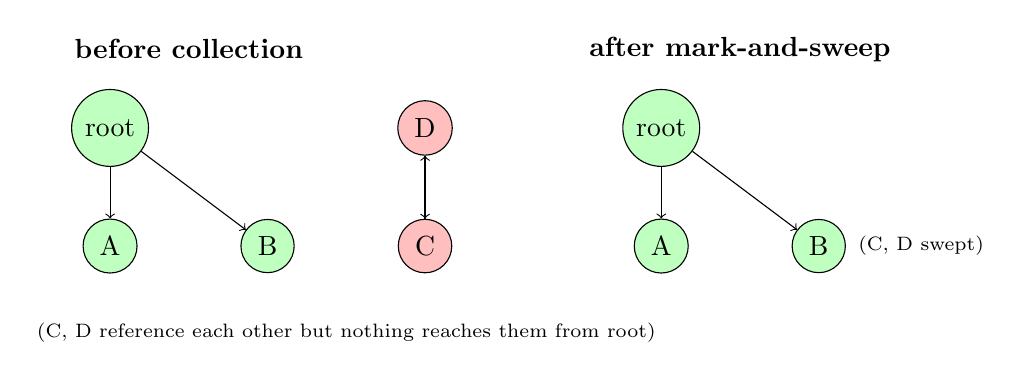
\begin{tikzpicture}[node distance=1.4cm]
  \node[font=\bfseries] (before) at (0,3) {before collection};
  \node[draw,circle,fill=green!25] (r1) at (-1,2) {root};
  \node[draw,circle,fill=green!25] (a1) at (-1,0.5) {A};
  \node[draw,circle,fill=green!25] (b1) at (1,0.5) {B};
  \node[draw,circle,fill=red!25]   (c1) at (3,0.5) {C};
  \node[draw,circle,fill=red!25]   (d1) at (3,2) {D};
  \draw[->] (r1) -- (a1);
  \draw[->] (r1) -- (b1);
  \draw[->] (c1) -- (d1);
  \draw[->] (d1) -- (c1);
  \node[font=\scriptsize] at (2,-0.6) {(C, D reference each other but nothing reaches them from root)};

  \node[font=\bfseries] (after) at (7,3) {after mark-and-sweep};
  \node[draw,circle,fill=green!25] (r2) at (6,2) {root};
  \node[draw,circle,fill=green!25] (a2) at (6,0.5) {A};
  \node[draw,circle,fill=green!25] (b2) at (8,0.5) {B};
  \draw[->] (r2) -- (a2);
  \draw[->] (r2) -- (b2);
  \node[font=\scriptsize] at (9.3,0.5) {(C, D swept)};
\end{tikzpicture}
\end{center}

Notice mark-and-sweep handles the cycle (C, D above) correctly, exactly where pure
reference counting failed: reachability from the roots, not mutual reference, is the
criterion, so an unreachable cycle simply never gets marked, and the sweep phase
reclaims it along with everything else that wasn't.

The cost mark-and-sweep leaves behind is \textbf{fragmentation}: the surviving objects
(A, B above) are left wherever they originally were in the heap, with holes where C and
D used to be. Over many collections, the heap can end up as live objects scattered
among many small unusable gaps, none individually large enough for a new, bigger
allocation, even though the total free space would be plenty if it were contiguous.

\subsection{mark-compact}

\textbf{Mark-compact} is mark-and-sweep's fix for exactly that fragmentation problem:
after marking, instead of just sweeping dead objects in place, it \emph{slides} the
surviving live objects together, so they end up contiguous, and updates every pointer
that referred to a moved object to point at its new location. You get a heap with no
gaps between live objects, at the cost of an extra pass (and the bookkeeping needed to
fix up every pointer to a moved object).

\subsection{copying collection and Cheney's algorithm}

\textbf{Copying (semispace) collection} takes a different approach: split the heap into
two equal halves, \emph{from-space} and \emph{to-space}. The program only ever
allocates in from-space. When it fills up, the collector walks the roots and copies
every \emph{live} object it finds over into to-space (leaving garbage behind,
un-copied, in from-space), then simply swaps the roles of the two halves, what was
to-space becomes the new from-space for the program to allocate into next.

\textbf{Cheney's algorithm} is the classic way to do this copy without needing a
separate, explicit stack to drive the traversal: it uses a scan pointer that walks
through to-space \emph{as objects are being copied into it}, and for each object it
scans, it copies (or finds already-copied) every object that one points to, advancing
the scan pointer as it goes, until the scan pointer catches up to the point where new
objects are being appended. The whole live set gets copied in one linear pass over
to-space, no recursion, no auxiliary stack.

Compaction comes essentially for free here: since you're only ever copying the objects
that are actually live, and packing them one after another as you copy them, the result
is automatically contiguous, with no separate compaction pass needed the way
mark-compact needs one. The catch is the name of the scheme itself: you only ever use
half the heap at any given time, the other half is sitting empty, reserved for the next
copy. For workloads with a lot of short-lived garbage (a large fraction of allocations
die almost immediately), this trade is a great one: copying is proportional to the
\emph{live} data, not the size of the heap, so if most things die young, most
collections are extremely cheap, you're barely copying anything. For workloads with
a lot of long-lived data, giving up half the heap is a real, painful cost.

\subsection{the generational hypothesis}

That last observation, ``a lot of short-lived garbage'' being the common case, has a
name: the \textbf{generational hypothesis}, most objects die young. Empirically, across
a huge range of real programs, the large majority of allocated objects become garbage
very quickly (a temporary string, a loop-local list, an intermediate result), while a
small minority stick around for a long time (long-lived caches, top-level data
structures).

\textbf{Generational GC} is built directly on that observation: split the heap into (at
least) a \textbf{young generation} and an \textbf{old generation}. New objects are
allocated in the young generation, and it's collected far more often than the old
generation, since if most objects there are about to die anyway, a young-generation
collection is cheap (little live data to copy or mark) and reclaims a lot of memory
per collection. An object that survives enough young-generation collections (some
threshold number) gets \textbf{promoted} into the old generation, on the theory that
anything that's survived that long is probably going to stick around, so it's not worth
re-scanning it on every cheap young collection. The old generation is collected only
occasionally, with a heavier full collection.

\subsection{the tri-color abstraction}

For reasoning about (and implementing) a tracing collector, especially one that runs
\textbf{concurrently} or \textbf{incrementally} alongside the running program (the
\textbf{mutator}, in GC terminology) rather than stopping it completely, the standard
mental model is the \textbf{tri-color abstraction}. Every object is, at any point during
a collection, one of:
\begin{itemize}
  \item \textbf{White}: not yet visited. At the start of a collection, everything is
    white. Anything still white at the end of marking is garbage.
  \item \textbf{Gray}: visited, known reachable, but its own outgoing pointers haven't
    all been scanned yet, it's ``on the frontier'' of the traversal.
  \item \textbf{Black}: visited, and every object it points to has also already been
    visited (scanned and colored gray or black).
\end{itemize}
Marking proceeds by repeatedly picking a gray object, scanning its pointers (coloring
any white targets gray), and then coloring the object itself black, until no gray
objects remain; whatever is still white at that point is unreachable.

The reason this abstraction matters especially for concurrent collectors: if the
mutator is allowed to keep running \emph{during} marking, it might write a pointer to
a white object into a black object's field, after that black object has already been
fully scanned. If nothing catches this, the white object stays white (looks
unreachable) even though a live, black object now points to it, and the collector will
incorrectly reclaim a live object. The standard fix is a \textbf{write barrier}: a
small piece of code the compiler inserts around every pointer-writing operation during
a concurrent collection, which notices exactly this situation (a black object about to
point at a white one) and re-colors something (typically the white target back to
gray) so it gets properly rescanned before the collection finishes. Write barriers are
the mechanism that keeps a concurrent collector's view of the heap consistent even
while the mutator is actively mutating pointers underneath it.

\subsection{Exercises}
\begin{itemize}
  \item Extend the two-object cycle example with a third object, \texttt{c}, so that
    \texttt{a}, \texttt{b}, and \texttt{c} form a three-cycle (\texttt{a.other = b},
    \texttt{b.other = c}, \texttt{c.other = a}) with no outside references. Trace the
    refcounts after all three names are deleted, and confirm none of them reach zero.
  \item Draw a mark-and-sweep before/after diagram (as in this section) for a heap with
    a root pointing to A, A pointing to B, and an unreachable pair C/D that reference
    each other, then a separate unreachable object E with no references at all. Which
    objects get marked? Which get swept?
  \item Trace Cheney's algorithm by hand on a tiny example: from-space contains
    reachable objects A (pointing to B) and B (pointing to nothing), plus unreachable
    garbage G. Show the order objects get copied into to-space and how the scan
    pointer advances.
  \item Think about it: why does the generational hypothesis specifically justify
    collecting the young generation \emph{more often} rather than just making the
    single, whole-heap collector faster in general? What would you lose by simply
    running one full mark-and-sweep pass more frequently instead of separating
    generations?
  \item In the tri-color abstraction, explain why an object can never go directly from
    black back to white without a write barrier's intervention, and why that specific
    transition (a black object gaining a pointer to a white one) is the dangerous case
    for a concurrent collector.
  \item Compare copying collection's ``give up half the heap'' cost against
    generational GC's promotion scheme. Could you combine them (e.g., use a
    copying collector specifically for the young generation)? What would justify that
    combination given what you know about the generational hypothesis?
\end{itemize}
